%\documentstyle[10pt,twoside]{article}
%\documentstyle[twoside]{article}
\documentclass[twoside]{article}
\setlength{\oddsidemargin}{0.25 in}
\setlength{\evensidemargin}{-0.25 in}
\setlength{\topmargin}{-0.6 in}
\setlength{\textwidth}{6.5 in}
\setlength{\textheight}{8.5 in}
\setlength{\headsep}{0.75 in}
\setlength{\parindent}{0 in}
\setlength{\parskip}{0.1 in}

\usepackage{graphicx}
\usepackage{url}


%
% The following commands sets up the lecnum (lecture number)
% counter and make various numbering schemes work relative
% to the lecture number.
%
\newcounter{lecnum}
\renewcommand{\thepage}{\thelecnum-\arabic{page}}
\renewcommand{\thesection}{\thelecnum.\arabic{section}}
\renewcommand{\theequation}{\thelecnum.\arabic{equation}}
\renewcommand{\thefigure}{\thelecnum.\arabic{figure}}
\renewcommand{\thetable}{\thelecnum.\arabic{table}}
\newcommand{\dnl}{\mbox{}\par}

%
% The following macro is used to generate the header.
%
\newcommand{\lecture}[4]{
   \pagestyle{myheadings}
   \thispagestyle{plain}
   \newpage
   \setcounter{lecnum}{#1}
   \setcounter{page}{1}
   \noindent
   \begin{center}
   \framebox{
      \vbox{\vspace{2mm}
    \hbox to 6.28in { {\bf CMPSCI~677~~~Operating Systems
                        \hfill Spring 2019} }
       \vspace{4mm}
       \hbox to 6.28in { {\Large \hfill Lecture #1: #2  \hfill} }
       \vspace{2mm}
       \hbox to 6.28in { {\it Lecturer: #3 \hfill Scribe: #4} }
      \vspace{2mm}}
   }
   \end{center}
   \markboth{Lecture #1: #2}{Lecture #1: #2}
   \vspace*{4mm}
}

%
% Convention for citations is authors' initials followed by the year.
% For example, to cite a paper by Leighton and Maggs you would type
% \cite{LM89}, and to cite a paper by Strassen you would type \cite{S69}.
% (To avoid bibliography problems, for now we redefine the \cite command.)
%
\renewcommand{\cite}[1]{[#1]}

% \input{epsf}

%Use this command for a figure; it puts a figure in wherever you want it.
%usage: \fig{NUMBER}{FIGURE-SIZE}{CAPTION}{FILENAME}
\newcommand{\fig}[4]{
            %\vspace{0.2 in}
            \centerline{\includegraphics[scale=#2]{#4}}
            \begin{center}
            Figure \thelecnum.#1:~#3
            \end{center}
    }

% Use these for theorems, lemmas, proofs, etc.
\newtheorem{theorem}{Theorem}[lecnum]
\newtheorem{lemma}[theorem]{Lemma}
\newtheorem{proposition}[theorem]{Proposition}
\newtheorem{claim}[theorem]{Claim}
\newtheorem{corollary}[theorem]{Corollary}
\newtheorem{definition}[theorem]{Definition}
\newenvironment{proof}{{\bf Proof:}}{\hfill\rule{2mm}{2mm}}

% Some useful equation alignment commands, borrowed from TeX
\makeatletter
\def\eqalign#1{\,\vcenter{\openup\jot\m@th
  \ialign{\strut\hfil$\displaystyle{##}$&$\displaystyle{{}##}$\hfil
      \crcr#1\crcr}}\,}
\def\eqalignno#1{\displ@y \tabskip\@centering
  \halign to\displaywidth{\hfil$\displaystyle{##}$\tabskip\z@skip
    &$\displaystyle{{}##}$\hfil\tabskip\@centering
    &\llap{$##$}\tabskip\z@skip\crcr
    #1\crcr}}
\def\leqalignno#1{\displ@y \tabskip\@centering
  \halign to\displaywidth{\hfil$\displaystyle{##}$\tabskip\z@skip
    &$\displaystyle{{}##}$\hfil\tabskip\@centering
    &\kern-\displaywidth\rlap{$##$}\tabskip\displaywidth\crcr
    #1\crcr}}
\makeatother

% **** IF YOU WANT TO DEFINE ADDITIONAL MACROS FOR YOURSELF, PUT THEM HERE:



% Some general latex examples and examples making use of the
% macros follow.

\begin{document}

%FILL IN THE RIGHT INFO.
%\lecture{**LECTURE-NUMBER**}{**DATE**}{**LECTURER**}{**SCRIBE**}
\lecture{4}{February 4}{Prashant Shenoy}{\textbf{Yi Fung}}

\section{Overview}
In the previous lecture, we learned about processes, processor scheduling, kernel-level threads, user-level threads, etc.  This lecture will cover the following topics:

\begin{description}
  \item[Multiprocessor scheduling] 
  \item[Distributed scheduling] 
  \item[Case Studies] : V-System, Sprite, Volunteer Computing, Condor
\end{description}

Q: Regarding the previous lecture, is the lightweight process that existed in Solaris operating system used in any other operating system nowadays?

A: Lightweight process does not exist exactly as it were designed, but many of the ideas carried over e.g. pthreads.

\section{Multiprocessor scheduling}
Here, we will talk about single machines with shared memory multiprocessor or multi-core CPU. Looking at the diagram below, the circles at the top are processors. Caches are presented at each of the processors. They keep instructions or data, and are used to speed up the execution of the program. There might be more than two level of caches (L1, L2, L3). Some caches are shared; others are not. Memory, or RAM, are shared across all of the processors using system bus; a program running on one processor can access any address in memory. Multi-processor scheduling involves scheduling tasks in such environment. 

\begin{center}
  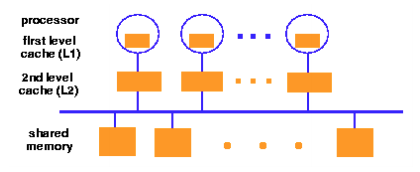
\includegraphics[scale=1]{multiprocessor_scheduling.png}\\
\end{center} 

\subsection{Central queue implementation}
In a central queue, all of the processors share a single ready queue where all the threads and processes are present. Whenever the time slice on any processor is going to end, that processor will look at the ready queue, pull a thread or process from that queue, and schedule it. 

\begin{center}
  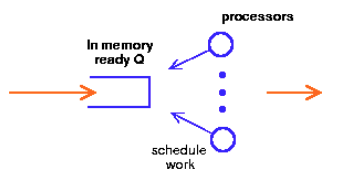
\includegraphics[scale=1]{central_queue.png}\\
\end{center} 

\subsection{Distributed queue implementation}
In a distributed queue, there are more than one queue in the system. The processes or threads are going to be part of one of those queue. When a processor becomes idle it is going to look at its local queue, and only take the next job in that queue to schedule for execution.

\begin{center}
  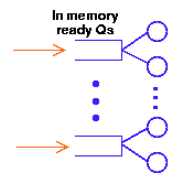
\includegraphics[scale=1]{distributed_queue.png}\\
\end{center} 

\subsection{Pros and cons of centralized queue and distributed queue}

The centralized queue is just shared data structure. As the number of processors grows, you have to use some synchronization primitives - the standard one being a lock. When the time slice on one processor ends, that processor has to go to the queue, lock the queue, and pick a job. If another processor becomes idle during this, this processor has to wait until the previous processor has picked the job and released the lock. No matter how efficient synchronization primitives are, there is still going to be synchronization overhead. That overhead will grow as the number of processors increases because there is going to be \textbf{lock contention}.

Distributed queue experiences less contention. When there is one queue per processor, there is hardly contention at all. The processor just goes to its local queue and pull a thread. Multiprocessor scheduling wouldn't be impacted by the \# of processors in a system.

But distributed queue needs to deal with \textbf{load imbalance}. Suppose there are n tasks. The n jobs will be split across the distributed queues. How splitting occur matters - if the queues are not equally balanced then some tasks are going to get more cpus time than others. Tasks in shorter queues get more round-robin timeshare. To deal with this, every once in a while look at all the queues and their lengths, and equalize them again so that every process gets approximately fair share of CPU time.

\textbf{Cache affinity} is important. Respecting cache affinity can hugely improve time efficiently. A process or thread has affinity to a processor because the cache there holds its data. Let\textsc{\char13}s say processor 1 picks up a job and schedules it for a time slice. By the time that time slice ends, the cache for that processor would be warm, with data and instruction for that job stored in the cache. The process goes to the end of the queue, eventually appears at the front, and get scheduled at another processor. There is no mapping of task to processor in the centralized queue. That processor will start from a cold cache, with no data and instruction for this job. The initial instructions will all be cache misses. Program execution is slowed down to warm up the cache, and then time slice ends.  

This argues using distributed queue based scheduling. Once process joins a queue it will stay in the same queue. Next time it gets scheduled there will be data and instructions from the previous time slice i.e. start with warm cache. But even though you might try to schedule process or thread on the same processor where it was executed last, every time you run again you still might not have all your data and instructions in the cache due to other processes in your system. You want to have larger time slices or quantum durations to account for the time when there is some early fraction of the quantum maybe all caches misses. You want to still get to run on the caches once it\textsc{\char13}s warmed up for some period of time. As a result, time slices in multiprocessor systems tend to be longer than the ones in uniprocessor systems. 

So, there are couple of things to keep in mind while scheduling on multiprocessors: 1. Exploit cache affinity: Try to schedule on the same processor that a process/thread executed last. 2. Pick larger quantum sizes for the time slicing to decrease context switch overhead.

\subsection{Scheduling parallel applications on SMP using gang scheduling}

One last point on multiprocessor scheduling. Until now, we assumed that the processes/threads are independent. We just picked the one at the front of the queue and we did not care about what was running in other processors. If you think of a parallel process with many many threads or a job with many processes that are coordinating some larger activities, you might not want to schedule them independently. For example, let\textsc{\char13}s say there are two cpu\textsc{\char13}s and a process with two threads. Let\textsc{\char13}s assume when these threads are executed they also need to communicate with each other for application needs. When T1 runs on Processor A, T2 may not be running on Processor B i.e. some other job may be running on Processor B. If T1 sends a message to T2, then it will wait for a reply until processor B runs T2 (so T2 can actually receive the message and process it). There is increase in waiting time. 

\begin{center}
  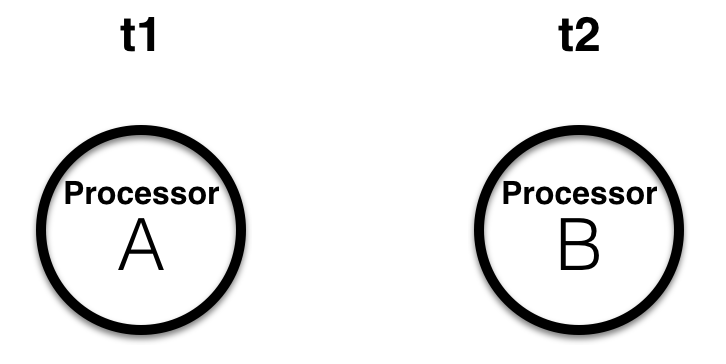
\includegraphics[scale=0.4]{cpu_process.png}\\
  Fig 1 : Two cpu, and a process with two threads.
\end{center} 

Gang scheduling schedule parallel jobs to run on different processors together, as a group in the same time slice. This allows true parallelism, i.e. all the threads of a process can run simultaneously. Gang scheduling is used in special-purpose multi-processors that are designed specifically to execute specialized, massively parallel applications such as scientific jobs.

Q: Is there a general purpose scheduling that you would normally run on a parallel machine and switch to gang scheduling only when there is a parallel application?

A: That is technically possible, but the hardware machines that gang schedulers run on are so specialized you would not run general-purpose applications.


\section{Distributed scheduling}

\subsection{Motivation}

Consider the scenario in which we have N independent machines connected to each other over a network. When a new application or process arrives at one of the machines, normally the operating system of that machine would execute job locally. In distributed scheduling, you have additional degree of flexibility. Even though the user submit job at machine i, the system may actually decides to execute the job at machine g and bring back the results. Distributed scheduling - taking jobs that are arriving at one machine and running them somewhere else in the system - does this makes sense (any advantage to this)?

\textbf{Scenario 1: Lightly loaded system utilization}
  
You should run job locally at the machine where it arrives. No benefit of moving a job because you have enough resources to do it.

\textbf{Scenario 2: Heavily utilized system}

You want to move a job somewhere else but there are no resources available in the system for you to run that job.
  
\textbf{Scenario 3: Moderately utilized system}

If a job arrives at machine i, and machine i happens to be slightly less loaded than other machines, then run it locally. If machine i happens to be more heavily loaded than other machines, then find another machine to run that job. This scenario would actually benefit from distributed scheduling.


\textbf{A more technical phrasing of the question would be}: \textit{what\textsc{\char13}s the probability that at least one system is idle and one job is waiting?} System idle means that exists some machine that has more resources to actually run more jobs than it is currently running. Job waiting means there is a job that arrived at heavily loaded machine and waiting to run. We benefit from distributed scheduling when both of these cases are true.

\begin{center}
  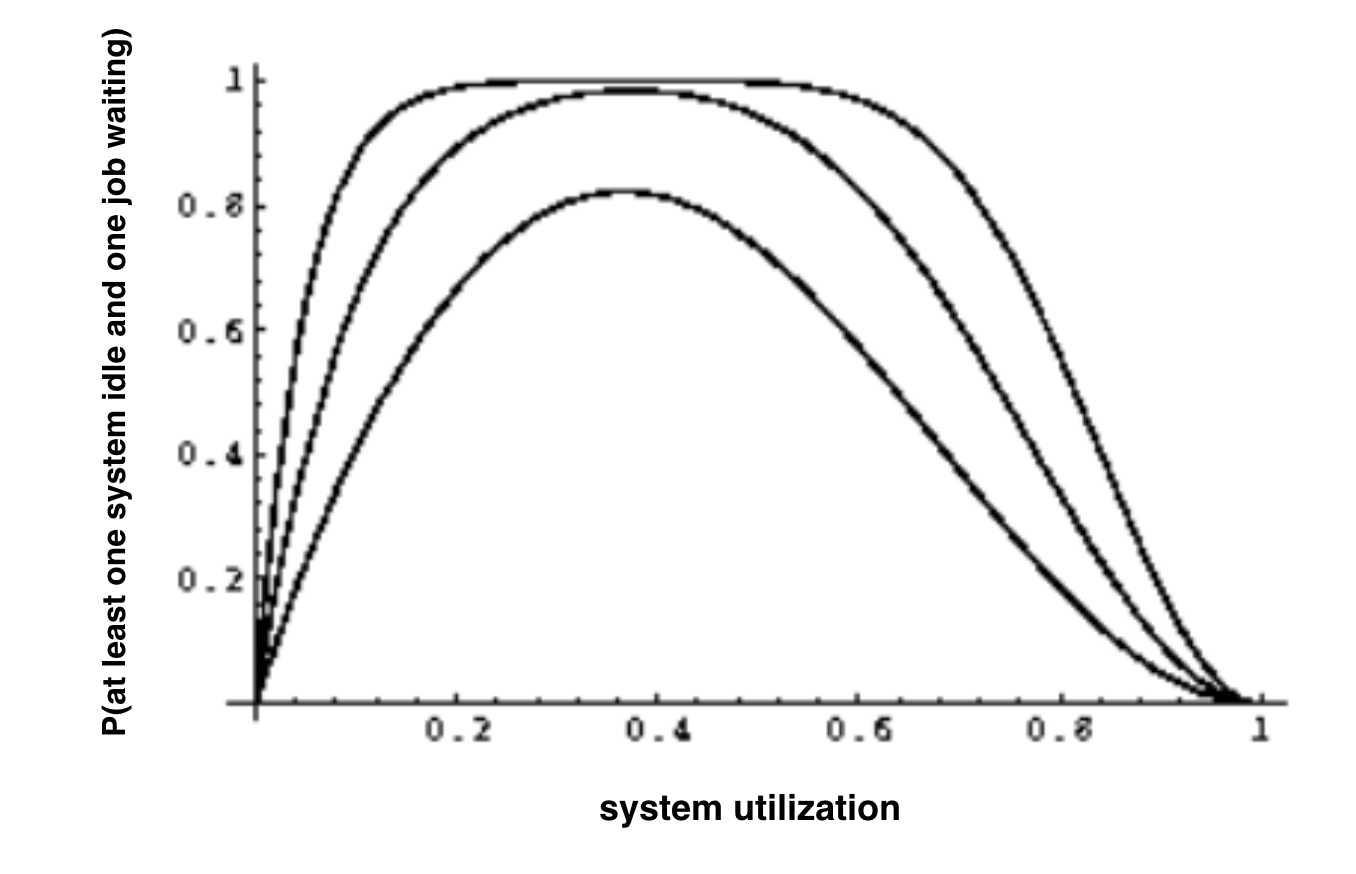
\includegraphics[scale=0.4]{pcurve.png}\\
\end{center} 

\begin{itemize}
\item {Lightly utilized system:  

P(at least one system idle)  high

P(one job waiting)  low

P(at least one system idle and one job waiting)  low} 

 \item {Heavily utilized system: 

P(one job waiting)  high

P(at least one machine idle)  almost zero

P(at least one system idle and one job waiting)  low}  

\item {Medium utilized system is the area of high probability under the curve
}
\end{itemize}

Note: P(at least one system idle and one job waiting) = P(one job waiting) * P(at least one system idle) 

The three lines are constructed by different system parameter settings but the overall curve is the point.

\subsection{Design issues}

{\bf Performance metric}: mean response time.\\

{\bf Load}: CPU queue length and CPU utilization. Easy to measure and reflect performance improvement. \\

{\bf Types of policies}: 
\begin{itemize}
\item {In \underline{static policy}, decisions are hard-wired into scheduling algorithm using prior knowledge of system.} 
\item {In \underline{dynamic policy}, the current state of the load information is used to dynamically make decisions.}
\item{In \underline{adaptive policy}, parameters of the scheduling algorithm change according to load. Can pick one of static or dynamic policy.}
\end{itemize} \\

{\bf Preemptive vs. Nonpreemptive}: 
\begin{itemize}
\item {\underline{Preemptive}  -- once job has started executing, scheduler can still preempt it and move somewhere else. Transfer of a partially executed task is expensive due to collection of task's state.} 
\item {\underline{Nonpreemptive} -- only transfer tasks that have not begun execution.}
\item {Preemptive schedulers are more flexible but complicated.}
 \end{itemize} \\

{\bf Centralized vs. Decentralized}: 
\begin{itemize}
\item {Centralized -- queue makes decision to send a job globally.}
\item {Decentralized -- queue makes decision locally.}
 \end{itemize} \\

{\bf Stability}: In queuing theory, the arrival rate should be less than system capacity or else the system will become unstable. When arrival rate is reaching system capacity, machines don't want incoming jobs and sends jobs off to other machines which also doesn't want them. Lots of processes are being shuffled around and nothing gets done. Queue starts building up, job floats around, system gets heavily loaded.

\subsection{Components of scheduler}

Distributed scheduling policy has 4 components to it.

i. {\bf Transfer policy} determines when to execute a process locally or transfer a process to some remote machine. Threshold-based transfer policies are commonly used to classify nodes as senders, receivers, or OK. \\

ii. {\bf Selection policy} determines which task should be transferred from a node. The simplest is to select a newly arrived task that have caused the node to become a sender. Moving processes that have already started executing is more complicated and expensive. The task selected for transfer should be such so that the overhead from task transfer is compensated by a reduction in task's response time.\\

iii. {\bf Location policy} determines where to transfer the selected task. This is done by polling
(serially or in parallel). A node can be selected for polling randomly, based on
information from previous polls, or based on nearest-neighbor manner. \\

iv. {\bf Information policy} determines when should information of other nodes be collected - demand-driven, periodic, or state-change-driven - so that the scheduler can make all of its decisions in the right way. \\

\subsection{Sender-initiated distributed scheduler policy}

\begin{center}
  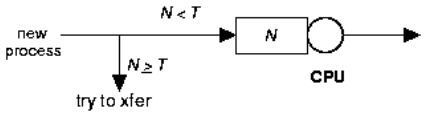
\includegraphics[scale=1]{senderinitiated.png}\\
\end{center} 

Overloaded node attempts to send tasks to lightly loaded node.
\begin{itemize}
\item {\bf Transfer policy}: CPU queue threshold, T, for all nodes. Initiated when a queue length exceeds T.
\item {\bf Selection policy}: newly arrived tasks. 
\item {\bf Location policy}:
\begin{itemize}
\item Random: select a random node to transfer the task. The selected node may be overloaded and need to transfer the newly arriving task out again. Is effective under light load conditions.
\item Threshold: poll nodes sequentially until a receiver is found or poll limit has been reached. Transfer task to the first node below threshold. If no receiver is found, then the sender keeps to the task.
\item Shortest: poll nodes in parallel and choose least loaded node below T. Marginal improvement.
\end{itemize}
\item {\bf Information policy}: demand-driven, initiated by the sender.
\item {\bf Stability}: Unstable at high-loads
\end{itemize}

\subsection{Receiver-initiated distributed scheduler policy}

Underloaded node attempts to receive tasks from heavily loaded node.
\begin{itemize}
\item {\bf Transfer policy}: when departing process causes load to be less than threshold T, node goes find process from elsewhere to take on.
\item {\bf Selection policy}:  newly arrived or partially executed process.
\item {\bf Location policy}:
\begin{itemize}
\item Random: randomly poll nodes until a sender is found, and transfer a
task from it. If no sender is found, wait for a period or until a task completes,
and repeat.
\item Threshold: poll nodes sequentially until a sender is found or poll limit is reached.
Transfer the first node above threshold. If none, then keep job.
\item Shortest: poll nodes in parallel and choose heaviest loaded node above T.
\end{itemize}
\item {\bf Information policy}: demand-driven, initiated by the receiver.
\item{\bf  Stability}: At high loads, a receiver will find a sender with a small number of polls with high-probability. At low-loads, most polls will fail, but this is
not a problem, since CPU cycles are available.
\end{itemize}

\subsection{Symmetrically-initiated distributed scheduler policy}

Sender-initiated and receiver-initiated components are combined to get a hybrid algorithm with the advantages of both. Nodes act as both senders and receiver. Average load is used as threshold. If load is below the average load, node acts as receiver. If load is above average threshold, node acts as sender.

\begin{center}
  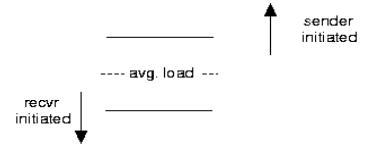
\includegraphics[scale=0.9]{symmetric1.png}\\
\end{center} 

Improved version exploit polling information to maintain sender, receiver, and OK nodes. Sender polls node on receiver list while receiver polls node on sender list.
\end{itemize}

\begin{center}
  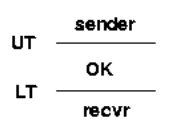
\includegraphics[scale=0.9]{symmetric2.png}\\
\end{center} 

Q: Isn\textsc{\char13}t there communication overhead?

A: Some; can broadcast your node and keep a table every minute or every time load changes. 

Q: How to pick threshold?

A: That\textsc{\char13}s configurable parameter; policy doesn\textsc{\char13}t care.

\section{Case Study}
\subsection{V-System}
Following a state-change driven information policy, the V-System broadcasts information when there is significant change in CPU/memory utilization. Nodes would listen to the broadcast and keep a load table. The V-System also implements a sender-initiated algorithm which maintains a list of M least loaded nodes. While off-loading, it probes a possible receiver randomly from M and transfers job only if it is still a receiver. When locating a node to receive job transferal, the system needs to double check whether the node on the list of M least loaded nodes is still a receiver because the load table is typically not updated super frequently unless policy did on-demand polling. One job is off-loaded at a time. 

\subsection{Sprite}
Sprite assumes a workstation environment in which ownership is king. When users are on their desktop they own it, and no other tasks will run on it. Other tasks can only run on desktops when there is no user using it. Like V-System, Sprite also uses state-change driven information policy and implements a sender-initiated scheduling algorithm. There is a centralized coordinator which keeps the status of load on all the machines. They made an assumption that if there is no mouse or keyboard activity for 30 seconds and the number of active processes is less than a threshold meaning there is at least one processor idle the node becomes a receiver. Foreign processes get terminated when the user returns. 

Q: Are the jobs exclusively CPU, or they can do I/O too?

A: They can do I/O. There is filesystem shared across all machines in some centralized server. 

Q: What if everybody goes to lunch (leave the machine idle) and comes back to work (use machine) at the same time?

A: There can be a queue of jobs awaiting execution, so they can be run on idle nodes when users are away. 

Sprite implemented process migration so that the process can suspend running job on a node and continue running from its last state at some other node, instead of killing and restarting the job. Process migration first stops a running job, writes out all registers and memory contents to disk, and transfers the entire memory contents as well as kernel state to receiver machine. Process migration is fairly complicated and comes with many problems e.g. I/O, network communication. Sprite comes at restriction and can only migrate certain types of process.

\subsection{Volunteer Computing}

Volunteer computing is based on the idea that PCs on the internet can volunteer to donate CPU cycles/storage when not in use and pool resources together to form an internet scale operating system.  A coordinator partitions a large job into small tasks and sends them to the volunteer nodes. Seti@home, BOINC and P2P backups are examples for this paradigm.

\subsection{Condor}

Condor makes use of idle cycles on workstations in a LAN. It can be used to run large batch jobs and long
simulations. It has a central job management system, called the condor, which idle machines contact to get assigned waiting jobs. It supports process migration and flexible job scheduling policies. The SLURM scheduler on UMass Swarm cluster is an example of this paradigm.

\end{document}
